\section{Introduction and EDA} \label{sec:eda}

\subsection{Problem Definition}
The task of the BigData Cup 2021 (Track 1) is to predict each user's feedback to 9 exposed items, given this user's click history, portrait features, and the items' features.
The special things about this task is that the 9 items are grouped into 3 sessions (\textit{c.f.} Figure \ref{fig:problemdef}). 
The user can only unlock the following session after he/she buys all 3 items in the previous session.

% \chen{input and output}

\begin{figure}[t!]
    \centering
    \includegraphics[width=\linewidth]{figures/problemdef.png}
    \caption{Problem Definition \cite{kaggle}}
    \label{fig:problemdef}
\end{figure}

%
\subsection{Exploratory Data Analysis (EDA)}
Before diving into the feedback prediction framework, we conduct exploratory data analysis firsthand to master the whole picture of the dataset.
\subsubsection{Data Statistics} \label{sec:eda:stats}

In total, there are 260,087 entries for training, and 206,254 entries for testing in track 1. 

% click
\para{Click} We first plot the histogram of how many times do each user clicked in Figure \ref{fig:analysis:click}. 
We can see that most of the users only click few times.

% buy
\para{Buy} We also plot the histogram of how many items do each user bought in Figure \ref{fig:analysis:buy}. 
We can see that 30912 users buy nothing, and 50267, 38191, 140717 users buy 1$\sim$3, 4$\sim$6, 7$\sim$9 items, respectively.
It is also interesting that very few people buy 3 or 6 items. We hypothesize that this is because the main reason why a user buy 3 or 6 items, is to unlock and buy the 3 items in the next session.
% sess
For the usage in the later paragraphs, we classify user states into 4 sessions:
\begin{itemize}
    \item sess0: user has bought 0 item.
    \item sess1: user has bought 1$\sim$3 items.
    \item sess2: user has bought 4$\sim$6 items.
    \item sess3: user has bought 7$\sim$9 items.
\end{itemize}
From Table \ref{tab:clickbuysess}, we can see that items in sess3 possess the majority of clicks and buys.


\begin{figure}
    \centering
    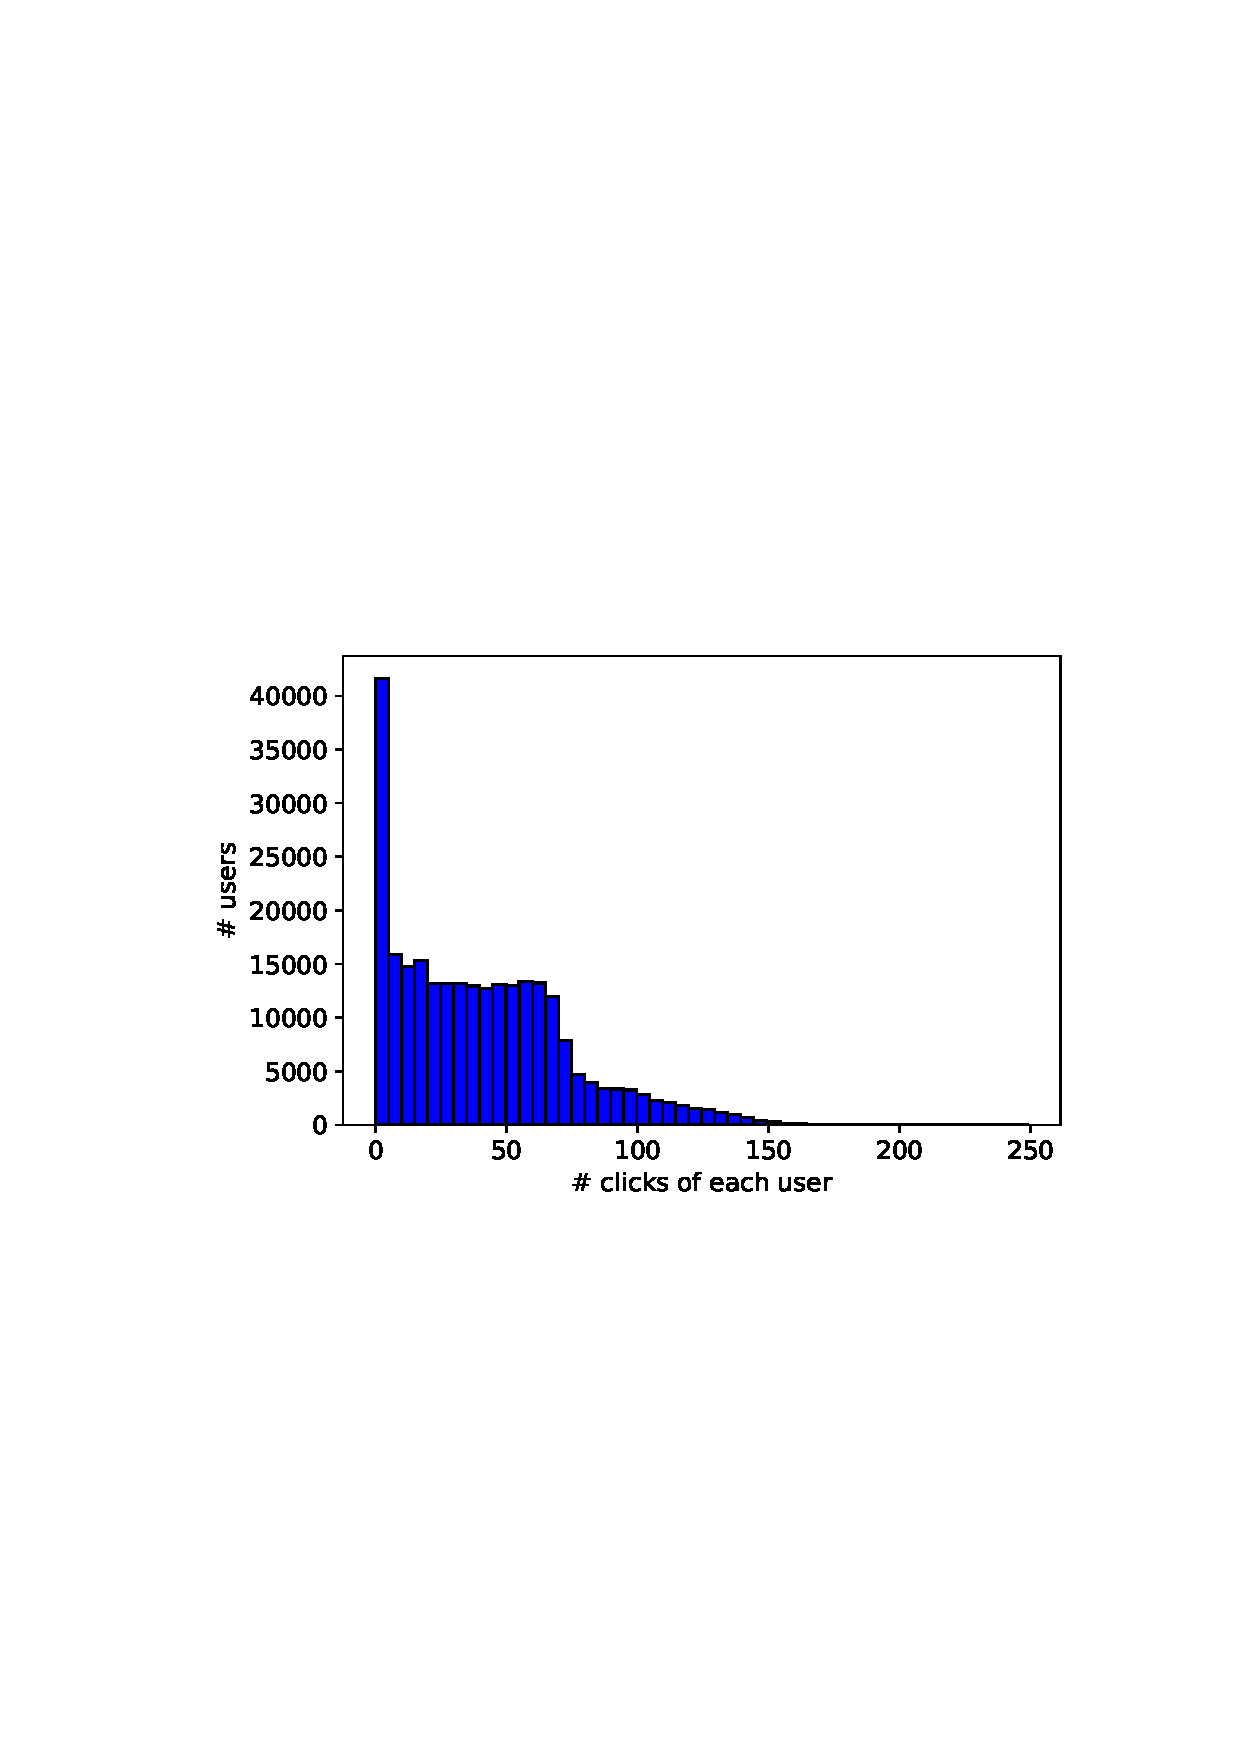
\includegraphics[width=\linewidth]{figures/analysis/click.png}
    \caption{Click Behavior}
    \label{fig:analysis:click}
\end{figure}

\begin{figure}
    \centering
    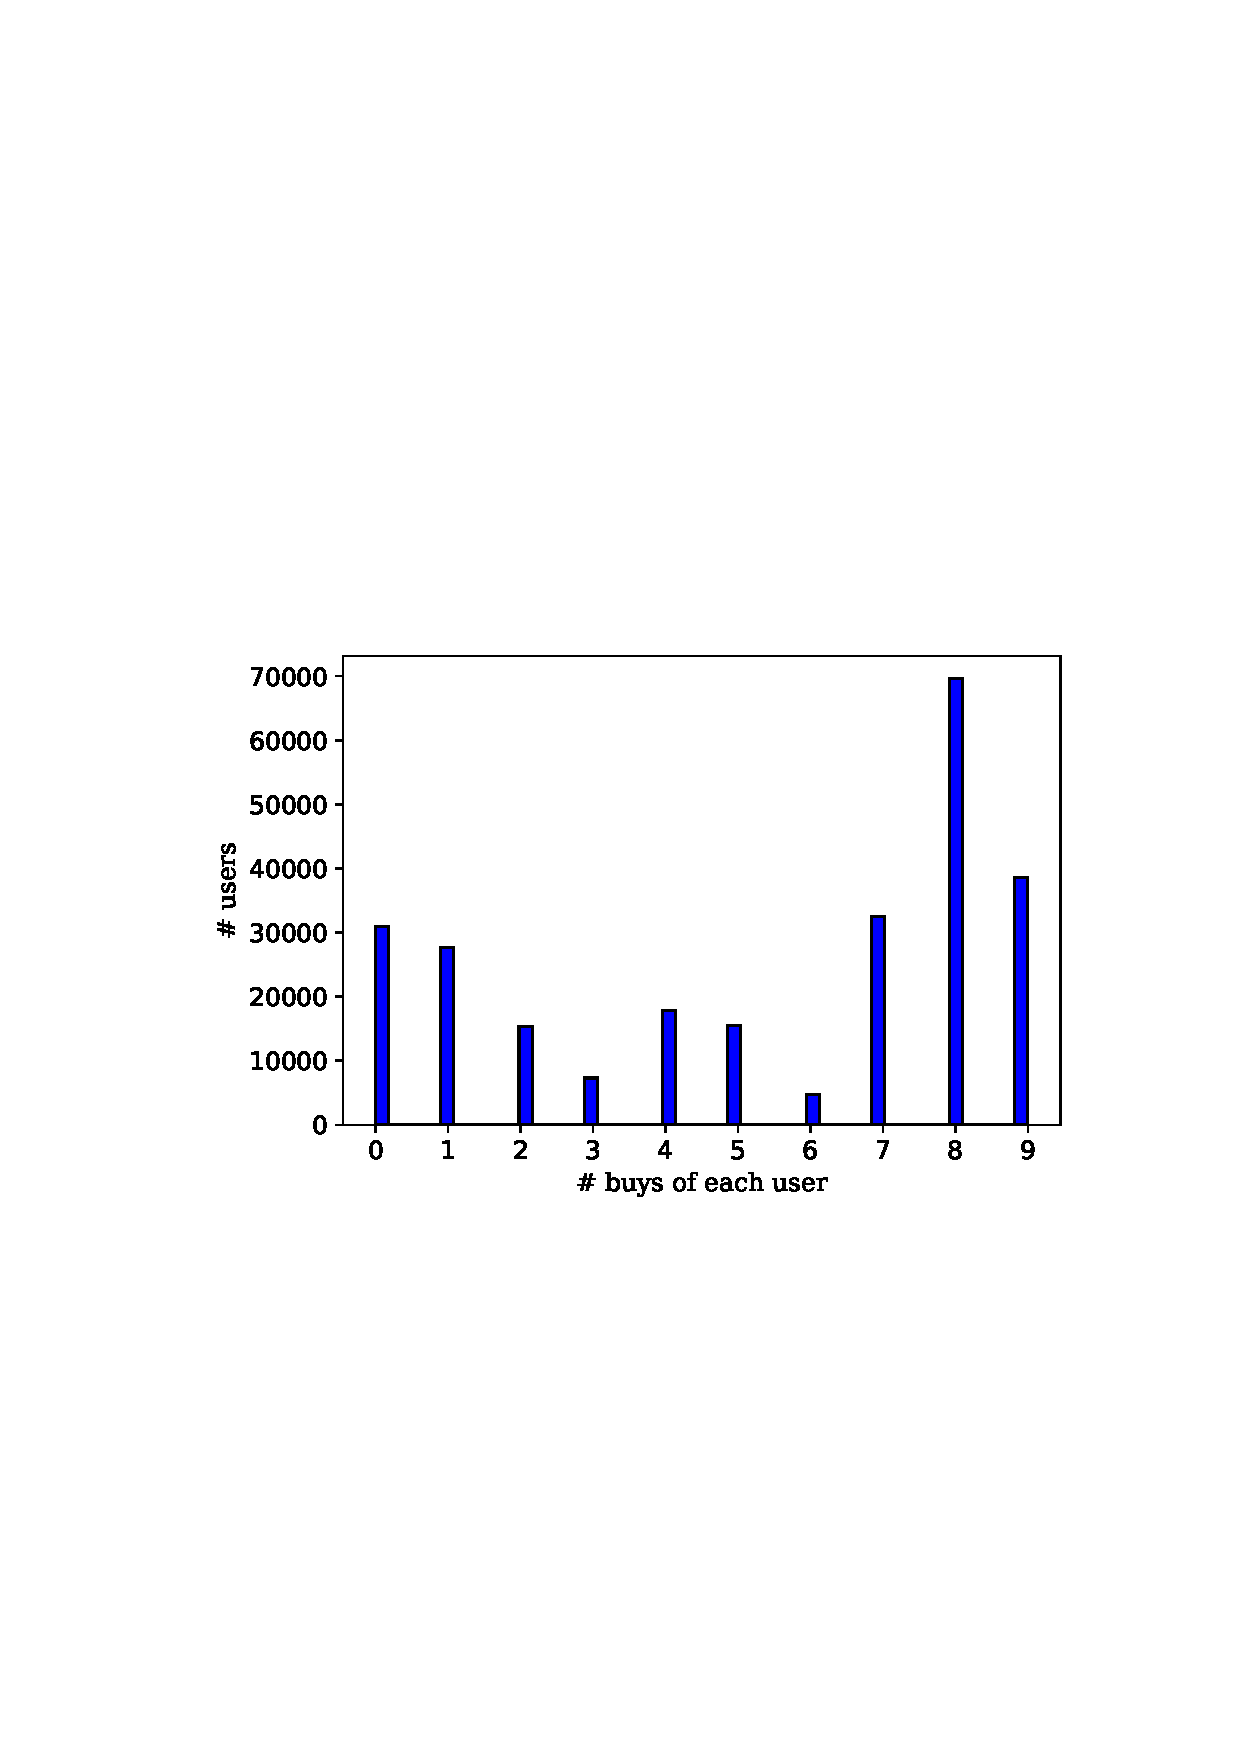
\includegraphics[width=\linewidth]{figures/analysis/buy.png}
    \caption{Buy Behavior}
    \label{fig:analysis:buy}
\end{figure}


\begin{table}[t!]
    \centering
    \caption{Click and Buy Statistics in Different Sessions.}
    \begin{tabular}{c|c|c|c} 
    \hline
    {\color[HTML]{333333} \textbf{Session}} & {\color[HTML]{333333} \textbf{Item IDs}} & {\color[HTML]{333333} \textbf{\# Clicks}} & {\color[HTML]{333333} \textbf{\# Buys}} \\ \hline
    {\color[HTML]{333333} 1} & {\color[HTML]{333333} 1$\sim$39 (39)} & {\color[HTML]{333333} 4,606,977} & {\color[HTML]{333333} 80,231} \\ \hline
    % \rowcolor[HTML]{333333} 
    {\color[HTML]{333333} 2} & {\color[HTML]{333333} 40$\sim$147 (108)} & {\color[HTML]{333333} 3,608,173} & {\color[HTML]{333333} 63,297} \\ \hline
    {\color[HTML]{333333} 3} & {\color[HTML]{333333} 148$\sim$381 (234)} & {\color[HTML]{333333} 2,220,648} & {\color[HTML]{333333} 287,482} \\ \hline
    \end{tabular}
    \label{tab:clickbuysess}
\end{table}


%%
\subsubsection{User Portrait and Item Features}
Since the meaning of user portrait features and item features are not given in the dataset description, we arrange their stats in Table \ref{tab:user_portrait} and Table \ref{tab:item_features}.
We can see that all user portrait are discrete features, while two of the item features are continuous features.



\begin{table*}[t!]
    \centering
    \caption{User portrait features.}
    \begin{tabular}{c|c|c|c|c|c|c|c|c|c|c}
    \hline
    {\color[HTML]{333333} \textbf{user\_portrait idx}} & 1 & {\color[HTML]{333333} \textbf{2}} & {\color[HTML]{333333} \textbf{3}} & {\color[HTML]{333333} \textbf{4}} & {\color[HTML]{333333} \textbf{5}} & {\color[HTML]{333333} \textbf{6}} & {\color[HTML]{333333} \textbf{7}} & {\color[HTML]{333333} \textbf{8}} & {\color[HTML]{333333} \textbf{9}} & {\color[HTML]{333333} \textbf{10}} \\ \hline
    {\color[HTML]{333333} \# unique\_values in trainset} & 3 & {\color[HTML]{333333} 1363} & {\color[HTML]{333333} 20} & {\color[HTML]{333333} 10} & {\color[HTML]{333333} 195} & {\color[HTML]{333333} 49} & {\color[HTML]{333333} 3} & {\color[HTML]{333333} 11} & {\color[HTML]{333333} 2} & {\color[HTML]{333333} 2164} \\ \hline
    {\color[HTML]{333333} \# unique\_values in testset\_track1} & 3 & {\color[HTML]{333333} 1319} & {\color[HTML]{333333} 19} & {\color[HTML]{333333} 10} & {\color[HTML]{333333} 191} & {\color[HTML]{333333} 47} & {\color[HTML]{333333} 3} & {\color[HTML]{333333} 13} & {\color[HTML]{333333} 2} & {\color[HTML]{333333} 2054} \\ \hline
    {\color[HTML]{333333} \# unique\_values in testset\_track2} & 3 & {\color[HTML]{333333} 1341} & {\color[HTML]{333333} 20} & {\color[HTML]{333333} 10} & {\color[HTML]{333333} 190} & {\color[HTML]{333333} 47} & {\color[HTML]{333333} 3} & {\color[HTML]{333333} 11} & {\color[HTML]{333333} 2} & {\color[HTML]{333333} 2060} \\ \hline
    \end{tabular}
    \label{tab:user_portrait}
\end{table*}



\begin{table*}[t!]
    \centering
    \caption{Item features.}
    \begin{tabular}{c|c|c|c|c|c}
    \hline
    {\color[HTML]{333333} \textbf{item\_feature idx}} & {\color[HTML]{333333} \textbf{1}} & {\color[HTML]{333333} \textbf{2}} & {\color[HTML]{333333} \textbf{3}} & {\color[HTML]{333333} \textbf{4}} & {\color[HTML]{333333} \textbf{5}} \\ \hline
    {\color[HTML]{333333} \# unique\_values in item\_info} & {\color[HTML]{333333} 4} & {\color[HTML]{333333} 10} & {\color[HTML]{333333} 2} & {\color[HTML]{333333} 241} & {\color[HTML]{333333} 214} \\ \hline
    % \rowcolor[HTML]{333333} 
    {\color[HTML]{333333} values} & {\color[HTML]{333333} 1,2,3,4} & {\color[HTML]{333333} 0,1,2,3,4,5,6,7,8,9} & {\color[HTML]{333333} 1,2} & {\color[HTML]{333333} 0$\sim$1, float} & {\color[HTML]{333333} 0$\sim$1, float} \\ \hline
    \end{tabular}
    \label{tab:item_features}
\end{table*}



% \chen{it seems that we have not summarized the conclusions of the EDA}